\subsection{\textit{Optimized link state routing} - OLSR}
O protocolo OLSR \'e um protocolo pr\'o-ativo
Pr\'o-ativo, marca\c{c}\~ao especial dos vizinhos.

\begin{figure}[H]
	\centering
	\subfigure[Primeiro est\'agio]{
		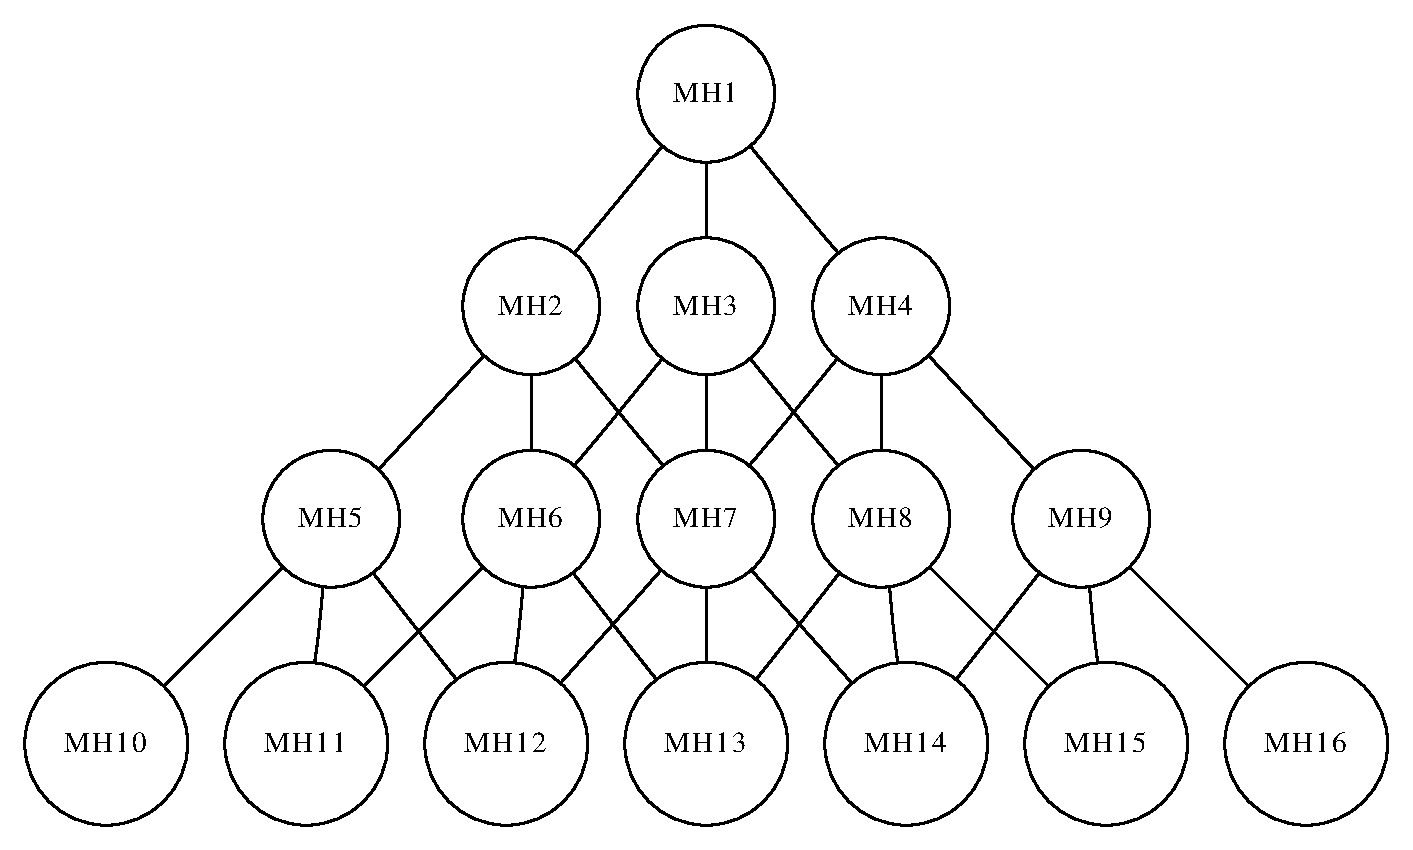
\includegraphics[scale=0.3]{olsrOperationStep1.eps}
	}\label{subfig:olsrStep11}
	\subfigure[Segundo est\'agio]{
		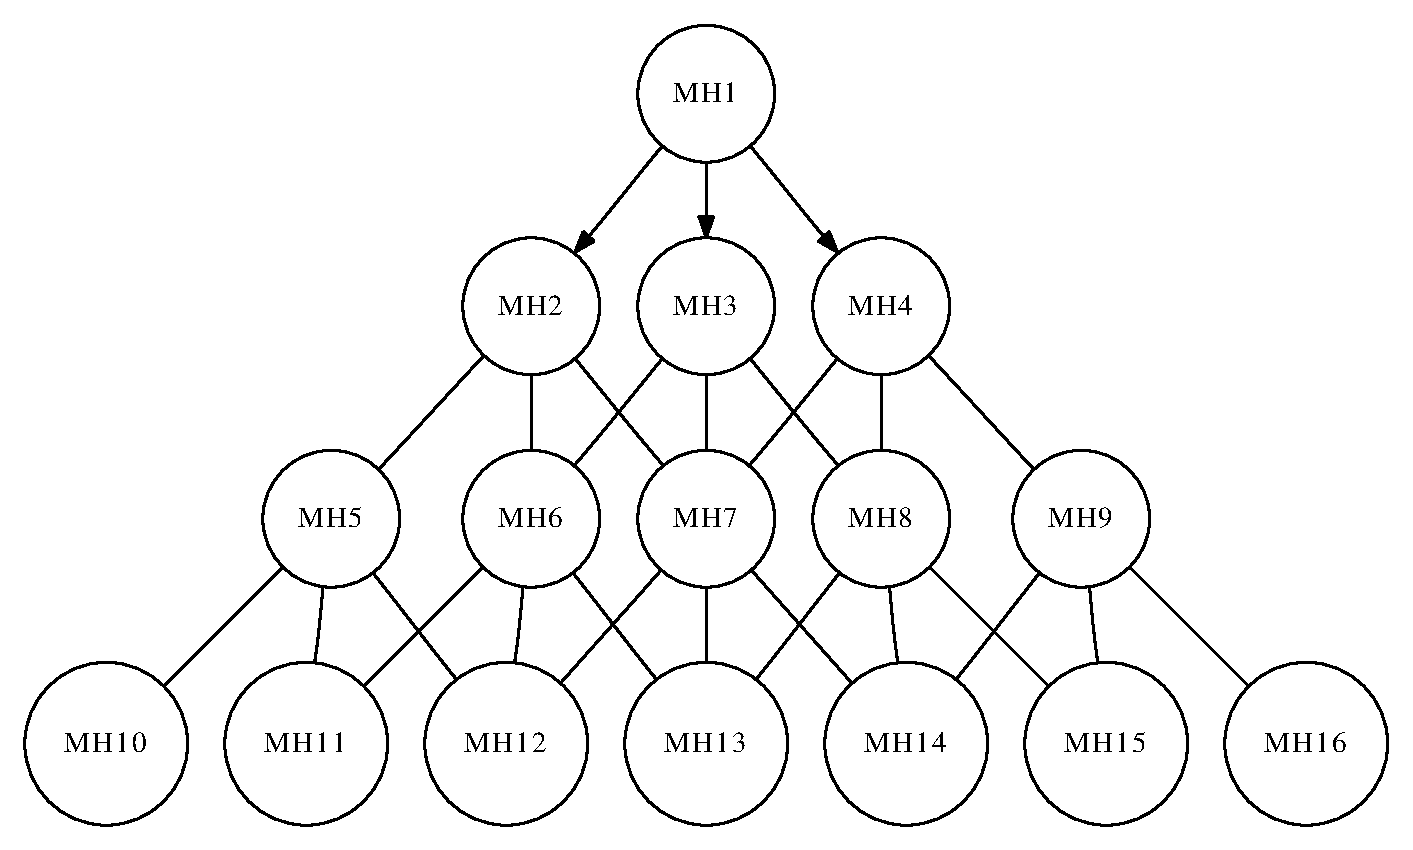
\includegraphics[scale=0.3]{olsrOperationStep2.eps}
	}\label{subfig:olsrStep12}
	\subfigure[Terceiro est\'agio]{
		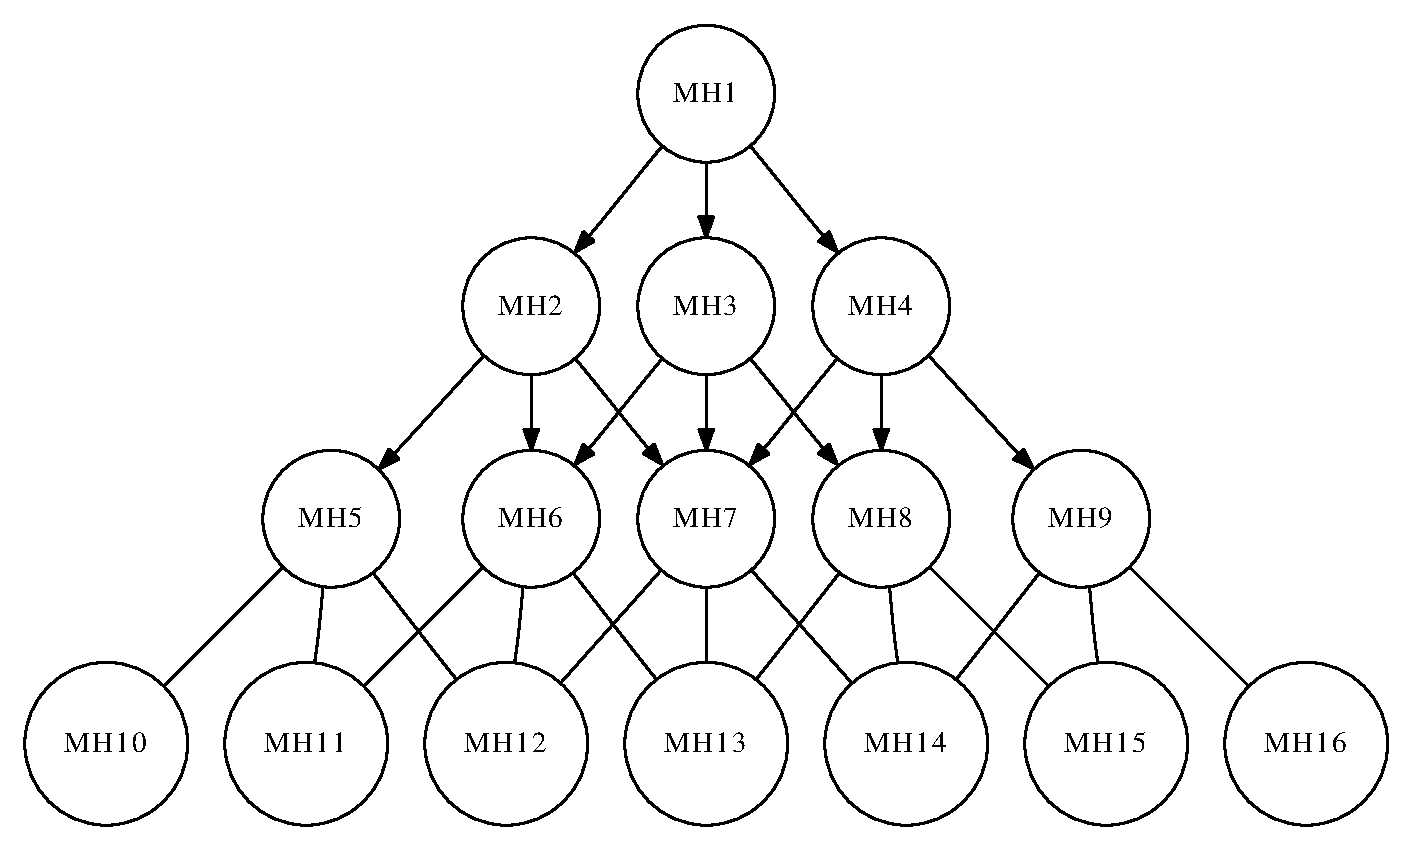
\includegraphics[scale=0.3]{olsrOperationStep3.eps}
	}\label{subfig:olsrStep13}
	\subfigure[Quarto est\'agio]{
		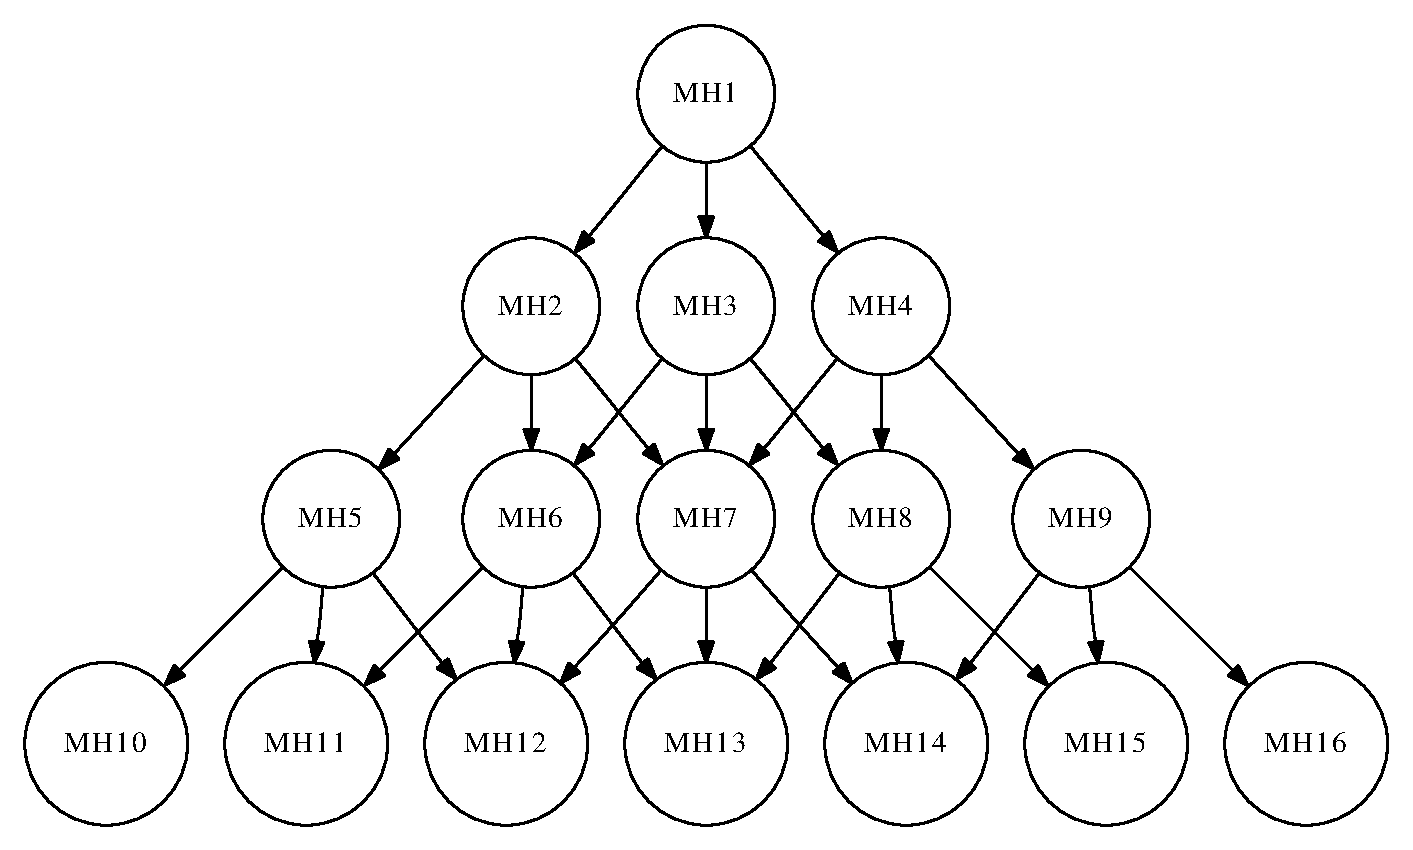
\includegraphics[scale=0.3]{olsrOperationStep4.eps}
	}\label{subfig:olsrStep14}	
	\caption{Descoberta de rotas de uma rede \textit{ad hoc} comum}
	\label{fig:olsrComum}
\end{figure}

\begin{figure}[H]
	\centering
	\subfigure[Primeiro est\'agio]{
		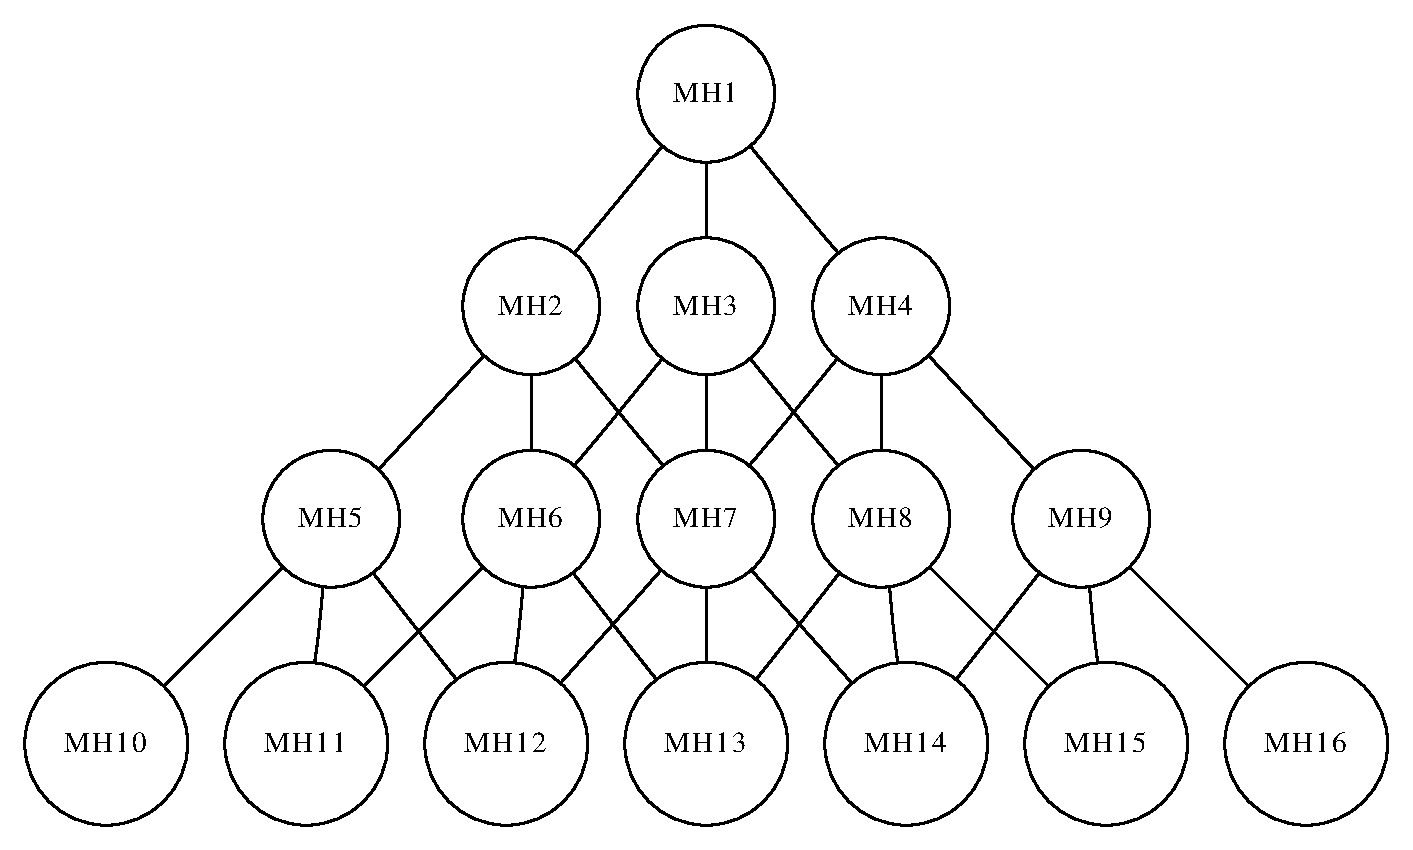
\includegraphics[scale=0.3]{olsrOperationStep1.eps}
	}\label{subfig:olsrStep21}
	\subfigure[Segundo est\'agio]{
		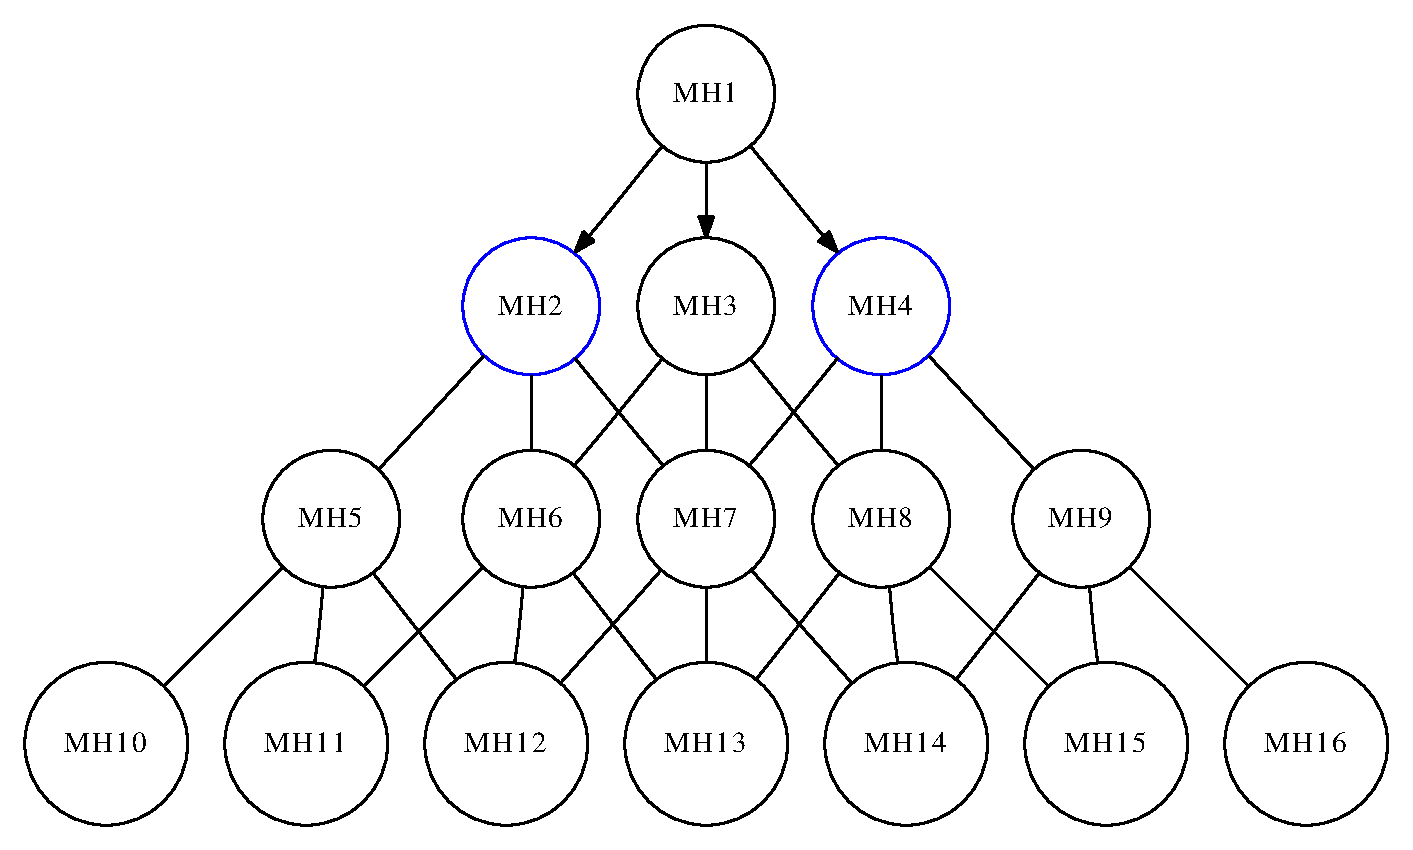
\includegraphics[scale=0.3]{olsrOperationStep5.eps}
	}\label{subfig:olsrStep22}
	\subfigure[Terceiro est\'agio]{
		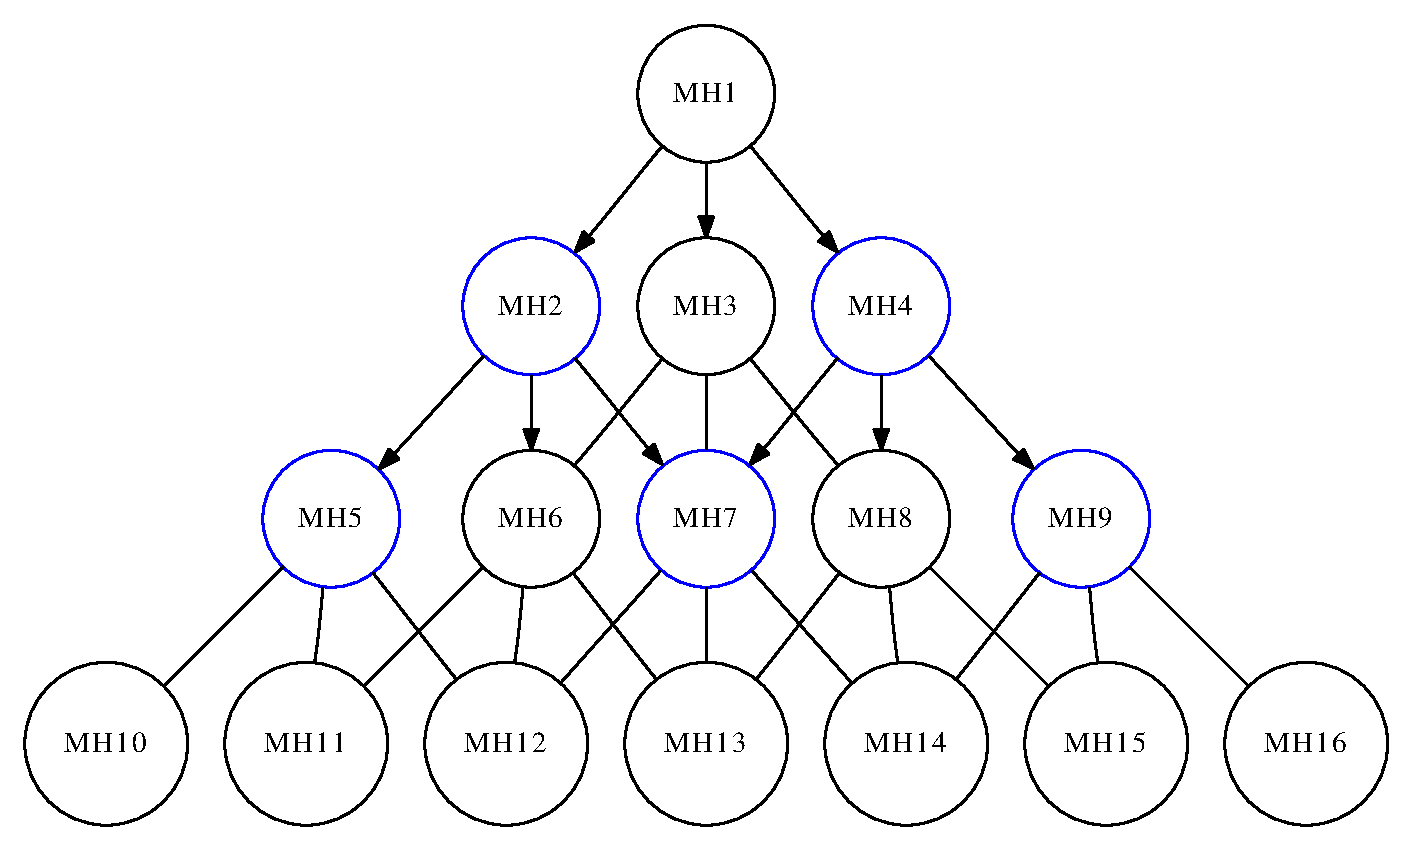
\includegraphics[scale=0.3]{olsrOperationStep6.eps}
	}\label{subfig:olsrStep23}
	\subfigure[Quarto est\'agio]{
		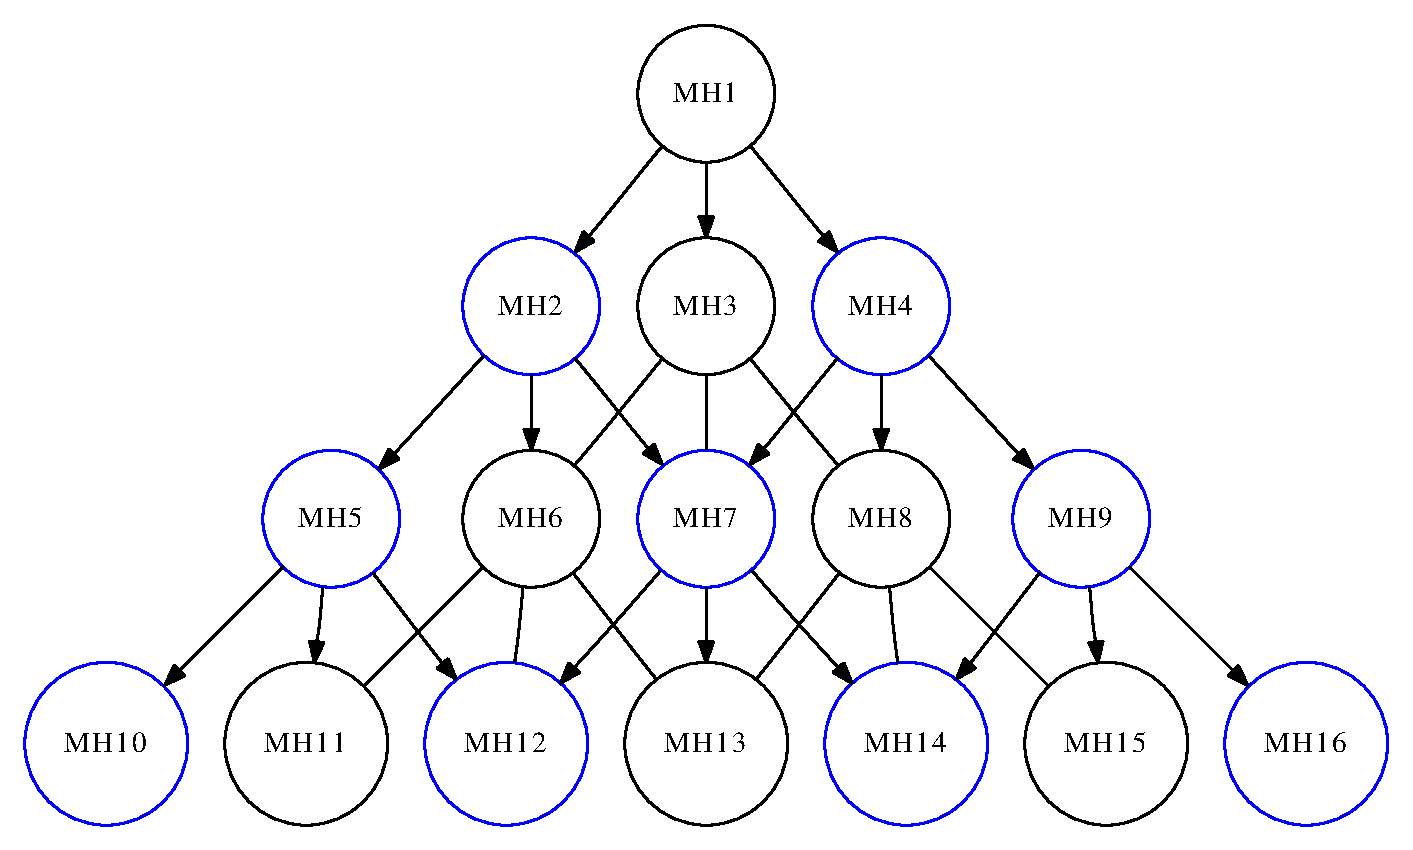
\includegraphics[scale=0.3]{olsrOperationStep7.eps}
	}\label{subfig:olsrStep24}	
	\caption{Descoberta de rotas do protocolo OLSR}
	\label{fig:olsrOperation}
\end{figure}
